
\begin{figure}
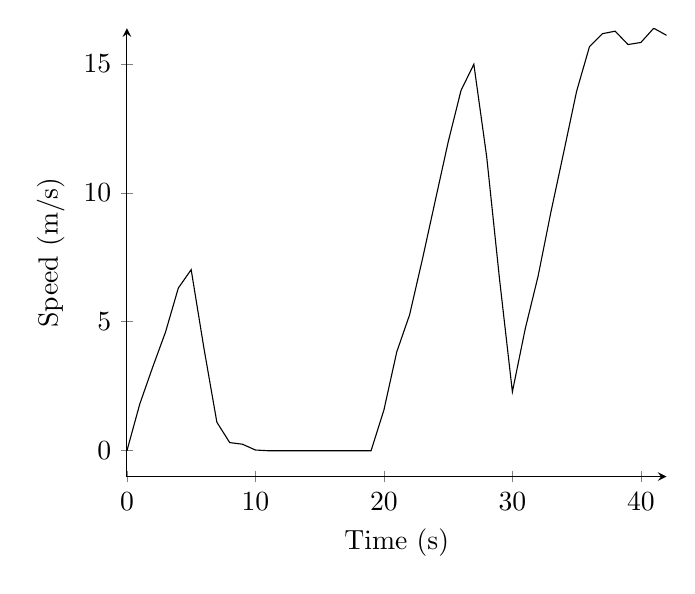
\begin{tikzpicture}
\begin{axis}[
legend style={
	anchor=west
},
axis x line=bottom,
axis y line=left,
ymin=-1,
point meta=explicit symbolic,
xlabel=Time (s),
ylabel=Speed (m/s)
]
\addplot[] coordinates {
(0, 0.0)
(1, 1.81086223427)
(2, 3.23543240374)
(3, 4.59506796265)
(4, 6.30643518205)
(5, 7.01996920655)
(6, 3.95487269728)
(7, 1.10602879862)
(8, 0.316181555033)
(9, 0.252501313198)
(10, 0.0284877896962)
(11, 0.0)
(12, 0.0)
(13, 0.0)
(14, 0.0)
(15, 0.0)
(16, 0.0)
(17, 0.0)
(18, 0.0)
(19, 0.0)
(20, 1.57842418179)
(21, 3.83097203478)
(22, 5.26943909237)
(23, 7.42986525089)
(24, 9.70187096653)
(25, 11.9617678673)
(26, 13.9643438335)
(27, 14.9819911091)
(28, 11.3957315998)
(29, 6.65159860662)
(30, 2.28642718309)
(31, 4.72785540154)
(32, 6.7642214728)
(33, 9.25548778872)
(34, 11.5834516153)
(35, 13.9387139753)
(36, 15.6646354519)
(37, 16.1666002476)
(38, 16.2644819103)
(39, 15.746840552)
(40, 15.826835368)
(41, 16.3793553953)
(42, 16.1040859008)
};

\end{axis}
\end{tikzpicture}
\label{tik:50:6_O, 6_O.-30, 7_S, 7_S.-25, 10_O}
\caption{50 percent diving with GSC on route $6_O, 6_O.-30, 7_S, 7_S.-25, 10_O$}
\end{figure}
